\documentclass[11pt]{article}
\usepackage[T1]{fontenc}
\usepackage[utf8]{inputenc}
\usepackage[english]{babel}
\usepackage{lmodern}
\usepackage[a4paper,margin=20mm]{geometry}
\usepackage{graphicx,booktabs,array,amsmath,amssymb,xcolor}
\usepackage{microtype}
\usepackage[colorlinks=true,linkcolor=teal,urlcolor=teal,citecolor=teal]{hyperref}
\definecolor{Ink}{HTML}{172B43}
\definecolor{Best}{HTML}{157553}
\definecolor{Rust}{HTML}{AF4D35}
\newcommand{\best}[1]{\textcolor{Best}{\textbf{#1}}}
\newcommand{\worst}[1]{\textcolor{Rust}{#1}}
\graphicspath{{figures/}}
\newcommand{\PCOne}{12.60}
\newcommand{\PCTwo}{7.69}
\newcommand{\PCTogether}{20.29}
\newcommand{\PCSelected}{91.50}

\setlength{\parindent}{0pt}
\setlength{\parskip}{5pt}
\newcommand{\figcaption}[1]{{\footnotesize #1\par}}
\newcommand{\topic}[1]{\par\medskip\textbf{#1}\par}

\hypersetup{pdftitle={Understanding dimensionality reduction in the NK-cell analysis},pdfauthor={SSBI group project}}
\begin{document}
\begin{center}
{\LARGE\bfseries Understanding dimensionality reduction}\par\medskip
{\large Methods, parameters and evidence in the NK-cell analysis}\par\smallskip
SSBI group project · Task 2 · 9 September 2026
\end{center}

\section*{1. What this analysis can answer}
The assignment asks us to visualise the provided data with PCA, t-SNE and UMAP, explain the effects of their parameters, show examples, and choose a quantitative measure for every pair of visualizations. These are questions about representations of the same observations. They are distinct from discovering validated cell populations or predicting the CMV status of previously unseen donors.

Horowitz et al. used mass cytometry to study variation in human natural killer (NK) cells. The original study involved 22 people; the provided project dataset contains 20 labelled donors. We analyse 37 selected protein markers, not 37 independent biological mechanisms. CyTOF distinguishes metal-isotope labels attached to antibodies and produces a marker-intensity vector for each cell. Marker intensities are informative about phenotype but do not directly measure whether a particular cell contains CMV.\cite{horowitz}

The later CellCNN study uses single-cell distributions to identify disease-associated subsets. It supplies the broader motivation for this group project: whether cellular patterns can help predict a donor-level outcome. Its results are not established again simply by producing a convincing two-dimensional map. The dimensionality-reduction task supplies exploratory views and measures of retained structure for the later clustering, classification and interpretation tasks.\cite{cellcnn}

\begin{center}
\begin{tabular}{lrp{.43\linewidth}}\toprule
Level & Size & Purpose\\\midrule
Provided gated NK data & 261,593 cells & Full reference for the sampling check\\
Balanced analysis data & 40,000 cells & 2,000 cells from each of 20 donors\\
Parameter-sweep sample & 5,000 cells & Fixed random subset of the balanced data\\
Distance-evaluation sample & 2,000 cells & Pairwise-distance correlations and Shepard plots\\\bottomrule
\end{tabular}
\end{center}

There are 9 CMV-positive and 11 CMV-negative donors in the provided labels. Each of the 40,000 analysis cells inherits its donor's label. These repeated labels do not create 40,000 independent clinical observations. The present notebook uses \texttt{gated\_NK}; it is an exploratory NK-cell analysis, not the \texttt{gated\_alive} main classification comparison specified for the later project task.

\topic{How to read this report}
Sections 2--4 explain preprocessing, sampling and PCA; Sections 5--8 explain t-SNE and UMAP; Sections 9--11 distinguish the evaluation measures; Sections 12--13 discuss biology, limitations and reproducibility. The paired short report is a one-page contribution to the shared report. This longer document is a separate explanation and preparation aid.

\clearpage
\section*{2. Why preprocessing changes the geometry}
For cell $i$ and marker $j$, let $x_{ij}$ be the raw intensity. The notebook applies the same cofactor $c=5$ to all markers:
\[
 a_{ij}=\operatorname{asinh}(x_{ij}/c)
 =\log\left(x_{ij}/c+\sqrt{1+(x_{ij}/c)^2}\right).
\]
Near zero, $\operatorname{asinh}(u)\approx u$, while for large positive $u$ it behaves approximately as $\log(2u)$. Unlike an ordinary logarithm, it is defined for zero and negative values and is an odd, monotone function. A positive cofactor cannot turn a positive measurement negative. The transform compresses the dynamic range while retaining the ordering of cells within each marker.

\begin{center}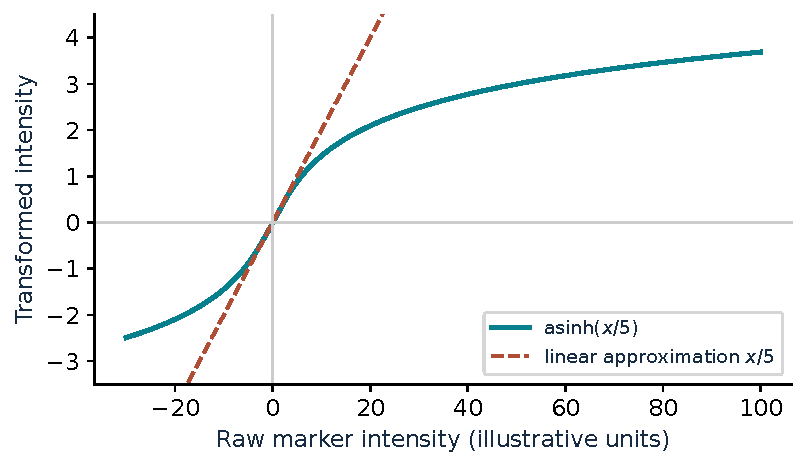
\includegraphics[width=.74\linewidth,height=56mm,keepaspectratio]{arcsinh.pdf}\end{center}
\figcaption{Figure 2. Mathematical illustration of arcsinh with cofactor 5 and its local linear approximation. The curve is not a fitted model or a new biological experiment.}

The cofactor sets the transition between approximately linear and approximately logarithmic behaviour. A larger cofactor leaves a wider raw-intensity range in the nearly linear regime. The notebook visually inspected cofactors 1, 3, 5, 8, 10 and 15 using CD3, CD56, CD16 and CD57. Its choice of 5 is a practical, qualitative choice; the histogram inspection is not an independently validated optimisation criterion. We should therefore not claim that this one value is optimal for every marker or that variance becomes constant by construction.

\topic{Variance filtering and z-scoring}
The notebook flags markers whose variance on the transformed scale is below 0.05. None is removed: all 37 remain. It then uses pooled marker-wise standardisation:
\[
 z_{ij}=\frac{a_{ij}-\bar a_j}{s_j},\qquad
 \bar a_j=\frac1n\sum_i a_{ij},\qquad
 s_j^2=\frac1{n-1}\sum_i(a_{ij}-\bar a_j)^2.
\]
This prevents markers with large numerical scales from dominating Euclidean distances. It also changes the relative contribution of markers: standardisation is a scientific choice, not a neutral cosmetic adjustment. It does not automatically correct batch effects or distinguish biological variability from technical variability.

The pooled scaling is appropriate to describe this fixed exploratory dataset. It must not be reused as a globally fitted preprocessing step inside a classification benchmark: in that setting, the means and scales must be learned using training donors only and applied unchanged to validation or test donors. No classification training is performed here.

\clearpage
\section*{3. What the subsampling check does and does not establish}
Taking an equal number of cells from each donor prevents donors with more recorded events from dominating the exploratory sample. For this dataset the chosen count is 2,000 per donor. Even balanced sampling can lose small populations, so the notebook checks one biologically motivated marker combination against the full gated NK dataset.

NKG2C$^+$/CD57$^+$ NK populations have been associated with prior CMV exposure and described as memory-like. ``Adaptive'' in this context refers to altered, potentially persistent response properties after immune experience; it does not mean that these cells have the rearranged antigen receptors of conventional adaptive lymphocytes. Co-expression of two markers is a phenotypic proxy, not a functional demonstration of memory or a proof of CMV infection of an individual cell.\cite{horowitz}

\begin{center}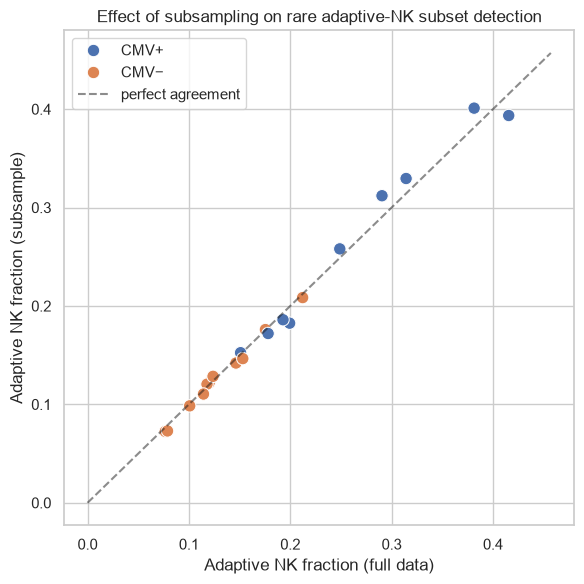
\includegraphics[height=69mm]{subsample.png}\end{center}
\figcaption{Figure 3. Original notebook output, cell 17. Each point is one donor; the dashed line is equal full-data and subsample fractions. Positivity thresholds are defined by the notebook's pooled two-component GMM procedure.}

\topic{How the positivity thresholds are obtained}
For each of NKG2C and CD57, a two-component Gaussian mixture is fitted to arcsinh-transformed values from all 261,593 NK cells. The component with the larger mean is called positive. A grid between the component means locates the first point where its posterior probability exceeds 0.5. This gives approximate transformed thresholds of 0.085845 and 0.084577, respectively. Cells above both thresholds are flagged, and the fraction is computed separately for each donor.

The fractions in the saved figure lie near the identity line, and the notebook reports no donor with fewer than ten flagged cells in the balanced sample. This supports retention of the particular GMM-defined fraction. It does not establish retention of all marker distributions, all rare subsets, or their joint structure. The plotted fraction is roughly 6--41\% within gated NK cells, so this phenotype is not necessarily rare in this restricted population even if related subsets are rare among all peripheral blood cells.

The GMM crossover depends on the assumed mixture shape and is not a validated manual gate. These pooled thresholds are used only for this descriptive check; using outcome information or held-out donors to learn a gate inside a prediction pipeline would require separate justification. No uncertainty intervals or repeated sampling study were added for the presentation.

\clearpage
\section*{4. PCA: a linear projection and an explicit variance budget}
Let $Z$ be the centred, standardised $n\times p$ matrix, here $n=40{,}000$ and $p=37$. PCA diagonalises the covariance matrix:
\[
 S=\frac{Z^\top Z}{n-1}=V\Lambda V^\top,
 \qquad Y_m=ZV_m,
 \qquad \lambda_1\ge\lambda_2\ge\cdots\ge0.
\]
The columns of $V_m$ are orthonormal loading vectors. Each score coordinate is a weighted sum of the marker values. PCA selects directions that maximise retained variance, equivalently minimising squared linear reconstruction error for a fixed number of components.

\begin{center}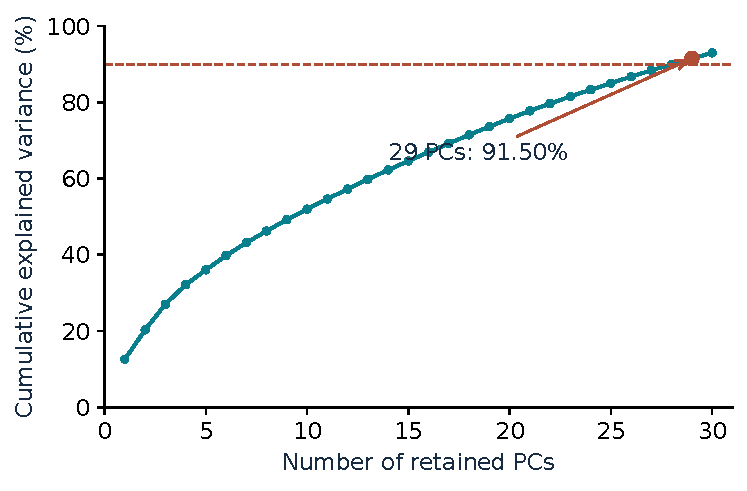
\includegraphics[height=57mm]{pca_spectrum.pdf}\end{center}
\figcaption{Figure 4. Cumulative explained variance, checked from the same standardised 37-marker matrix. The notebook initially fits 30 PCs and retains the first 29 at the 90\% threshold. This is a cumulative-variance plot rather than a search for an unambiguous elbow.}

The cumulative proportion is $C_m=\sum_{j=1}^m\lambda_j/\sum_{j=1}^p\lambda_j$. Here $C_{29}=0.914978$, whereas $C_2=0.202911$. PC1 contributes 12.60\% and PC2 contributes 7.69\%. Thus retaining 29 PCs for downstream calculations and displaying two PCs answer different questions. A weak separation in the first two axes does not establish the absence of structure elsewhere in the retained space.

\topic{What can be chosen?}
The number of retained components is the main investigated PCA parameter. The displayed axis pair is a separate choice. Preprocessing, numerical solver and whitening also matter. The notebook uses ARPACK, computes 30 components and does not whiten. Whitening would rescale retained PCs to equal variance and therefore alter the distances given to t-SNE or UMAP. None of these alternatives was systematically compared here.

\topic{Explained variance versus reconstruction error}
For $\widehat Z_m=Y_mV_m^\top$ and an MSE averaged over all matrix entries,
\[
 \frac{\lVert Z-\widehat Z_m\rVert_F^2}{np}
 =\frac{n-1}{n}\left(1-C_m\right)
\]
when each marker has unit sample variance. The small $(n-1)/n$ factor distinguishes MSE from the residual variance fraction. Both round to 0.0850 at 29 PCs here. They are derived from the same spectrum and should not be presented as independent evidence.\cite{pcaapi}

\clearpage
\section*{5. t-SNE: preserving probabilistic neighbourhoods}
t-SNE begins with pairwise similarities rather than directly minimising coordinate reconstruction error. For each point $x_i$ in the 29-PC input, it defines a conditional distribution over other observations:
\[
 p_{j|i}=\frac{\exp[-\lVert x_i-x_j\rVert^2/(2\sigma_i^2)]}
 {\sum_{k\ne i}\exp[-\lVert x_i-x_k\rVert^2/(2\sigma_i^2)]},\qquad p_{i|i}=0.
\]
The bandwidth $\sigma_i$ adapts to the local density. It is chosen to achieve a specified perplexity,
\[
 \operatorname{Perp}(P_i)=2^{H(P_i)},\qquad
 H(P_i)=-\sum_jp_{j|i}\log_2p_{j|i}.
\]
A distribution equally spread over $q$ neighbours has perplexity $q$. Real distributions are not uniform, so perplexity is an effective neighbourhood size rather than a literal instruction to retain exactly that many nearest neighbours. The directed probabilities are symmetrised as $p_{ij}=(p_{j|i}+p_{i|j})/(2n)$.

In the two-dimensional map, t-SNE uses a heavy-tailed Student kernel:
\[
 q_{ij}=\frac{(1+\lVert y_i-y_j\rVert^2)^{-1}}
 {\sum_{k\ne l}(1+\lVert y_k-y_l\rVert^2)^{-1}},\qquad q_{ii}=0.
\]
Optimisation minimises
\[
 C=\operatorname{KL}(P\|Q)=\sum_{i\ne j}p_{ij}\log\frac{p_{ij}}{q_{ij}}.
\]
If a pair is important in the original neighbourhood distribution but assigned very low probability in the map, it contributes strongly to the loss. The heavy tail allows moderately separated high-dimensional neighbourhoods more room in the map and helps alleviate the crowding problem. The gradient balances attraction associated with $P$ and repulsion associated with $Q$.\cite{tsne}

\topic{Why distances and island sizes need care}
The algorithm adapts neighbourhood bandwidths to density. A dense original group can expand and a sparse one contract in the map. Equal-looking areas therefore need not represent equal original density, and the distance between separated islands is not automatically a faithful original-space distance. Orientation has no intrinsic meaning. Local structure may look compelling even when a global shape comparison gives a poor fit.

The objective is non-convex and depends on initialisation and optimisation settings. A fixed seed supports reproducibility within a specified software environment; it does not show that the same visual structure appears for other seeds or implementations. A visually separated region should be checked using marker expression and independent analysis rather than named as a cell type from its shape alone.

\topic{Connection to the present task}
PCA supplies a 29-dimensional input with 91.50\% retained variance. The parameter sweep tests neighbourhood scale on 5,000 fixed cells. The selected setting is then used in the stored 40,000-cell t-SNE map. Sweep scores and final scores are therefore measurements at different sample sizes and cannot be treated as paired estimates of a performance improvement.

\clearpage
\section*{6. t-SNE: what was varied and what was fixed}
The sweep draws 5,000 cells without replacement from the balanced 40,000-cell dataset, using seed 42. All 20 donors remain represented, with 220--281 cells each. The sweep is therefore approximately, not exactly, balanced by donor. Every tested configuration uses the same cells in the same order and the same 29-PC input.

\begin{center}
\begin{minipage}{.56\linewidth}\centering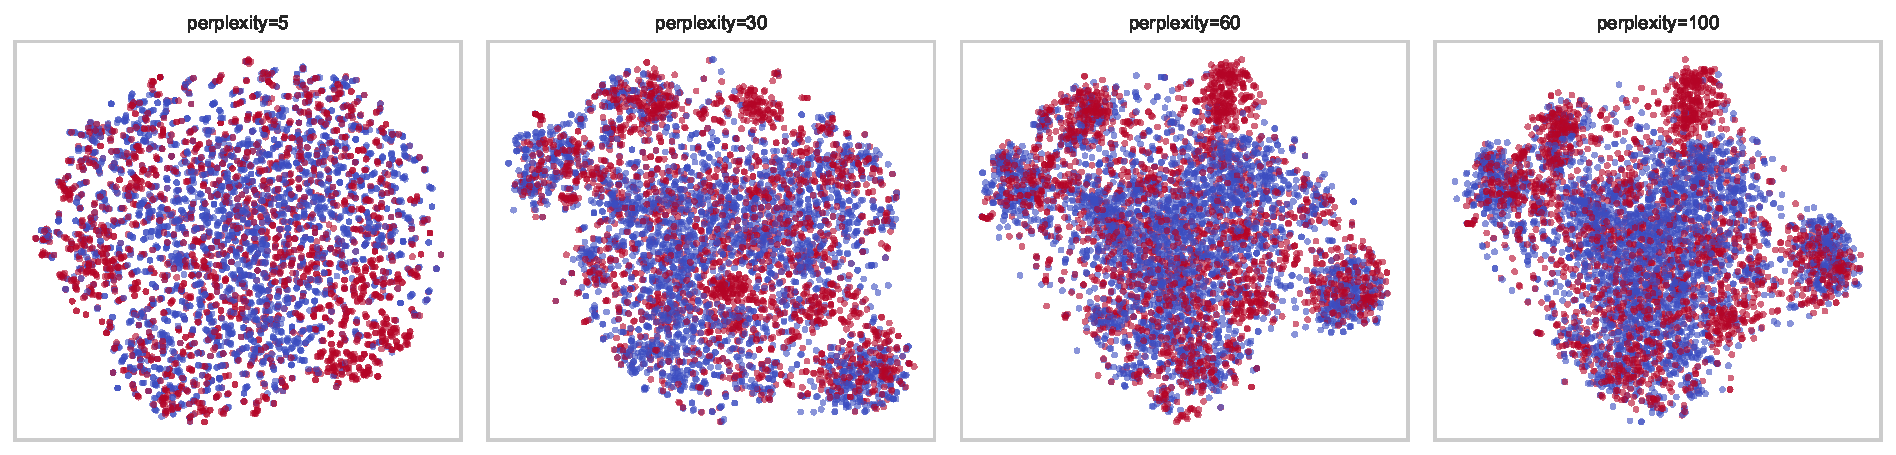
\includegraphics[width=\linewidth,height=66mm,keepaspectratio]{tsne_selected.pdf}\end{minipage}\hfill
\begin{minipage}{.37\linewidth}\centering\begin{tabular}{rr}\toprule
Perplexity & $T(15)$\\\midrule
5 & 0.894570\\
30 & 0.923184\\
50 & 0.925973\\
60 & 0.926046\\
70 & 0.924079\\
100 & 0.925800\\
\bottomrule\end{tabular}
\end{minipage}
\end{center}
\figcaption{Figure 5 and Table 2. Original panels for perplexities 5, 30, 60 and 100; complete saved Trustworthiness table. Blue/cyan denote CMV-negative/positive labels in these source panels. Invalid stored sweep kNN values are omitted.}

Perplexity 5 produces a more diffuse appearance in the saved panels; several larger settings show more distinct regions. The relevant observation is the actual change in these plots, not a universal rule that low perplexity must produce small islands. Perplexity 60 has the highest saved Trustworthiness, 0.926046, compared with 0.925973 at 50 and 0.925800 at 100. The gap between 50 and 60 is 0.000073, or 0.0073 percentage points. No repeated-seed experiment establishes that this ordering is stable.

\topic{Settings held fixed}
The notebook requests two output dimensions, PCA initialisation, random seed 42, 750 iterations and the Barnes--Hut approximation. It leaves Euclidean distance, early exaggeration 12, automatic learning rate and Barnes--Hut angle 0.5 at the documented scikit-learn defaults. In this implementation, the automatic learning rate is $\max(n/(4\,\text{early exaggeration}),50)$: about 104.2 for 5,000 points and 833.3 for 40,000 points. Defaults are version-dependent and should be recorded with the environment.\cite{tsneapi}

Early exaggeration strengthens attraction early in optimisation; learning rate controls step size; the number of iterations limits optimisation time; initialisation and seed affect the starting configuration; the approximation angle trades computational cost against force-approximation accuracy. Changing the input metric would change the neighbourhood problem itself. These parameters were held fixed to keep the experiment small and interpretable, not because they cannot alter the map. A fixed iteration budget is not proof of convergence.

The selection code ranks only Trustworthiness. It does not jointly optimise Trustworthiness and kNN preservation. The initially stored kNN table favoured perplexity 50, but those kNN values were affected by an implementation error and cannot establish a valid competing optimum. The corrected presentation retains the documented Trustworthiness-based choice and makes no claim about a corrected sweep-wide kNN winner.

\clearpage
\section*{7. UMAP: from a local graph to low-dimensional coordinates}
UMAP constructs a weighted graph representing local connectivity. A simplified description starts from distances to neighbouring observations. For point $i$, a local offset $\rho_i$ accounts for connectivity to its nearest neighbours, and a scale $\sigma_i$ adapts the decay of edge strength to local sampling density:
\[
 w_{j|i}=\exp\!\left[-\frac{\max(0,d(x_i,x_j)-\rho_i)}{\sigma_i}\right].
\]
These directed neighbourhood weights are combined using the fuzzy-union rule
\[
 w_{ij}=w_{j|i}+w_{i|j}-w_{j|i}w_{i|j}.
\]
Consequently, a strong relation in either local view contributes to a symmetric graph. The construction emphasises local connectivity and uses density adaptation; it is not simply a graph of unmodified Euclidean distances. The full mathematical framework is developed in the UMAP paper.\cite{umap}

In the map, a common expression for the low-dimensional edge weight is
\[
 v_{ij}=\left(1+a\lVert y_i-y_j\rVert^{2b}\right)^{-1},
\]
where $a$ and $b$ are set using the requested min\_dist and spread. A conceptual cross-entropy objective, omitting terms constant with respect to $Y$, is
\[
 L(Y)=-\sum_{i<j}\left[w_{ij}\log v_{ij}+(1-w_{ij})\log(1-v_{ij})\right].
\]
Large graph weights favour attraction, while non-neighbour relations contribute repulsion. Implementations use stochastic optimisation and negative sampling rather than materialising and optimising every possible pair in this expression. This distinction matters: the formula explains the intended graph-matching problem, not every detail of the optimiser's effective weighting.\cite{umapdocs}

\topic{How it differs from t-SNE}
Both methods use local similarities, permit nonlinear maps and optimise coordinates. Perplexity and n\_neighbors both control a neighbourhood scale, but they enter different constructions and are not interchangeable values. t-SNE forms entropy-controlled probability distributions and minimises KL divergence; UMAP constructs a locally scaled fuzzy graph and embeds it using a cross-entropy-inspired objective. Neither method guarantees that all long-range distances survive.

\topic{What a map can hide}
A two-dimensional representation must discard information when the data require more dimensions. Local density adaptation, the graph construction and the low-dimensional attraction/repulsion balance all affect the visible layout. A compact island can reflect a real coherent neighbourhood, a parameter choice, or both. Conversely, connected-looking regions can contain important variation in markers not visible on the two plotted axes.

The practical interpretation should therefore combine the parameter examples, numerical preservation measures and marker overlays. The notebook's final UMAP uses the selected 29-PC representation and produces coordinates for the same 40,000 cells shown in the PCA and t-SNE maps. This shared identity and ordering make the subsequent pairwise comparisons meaningful.

\clearpage
\section*{8. UMAP parameters and the observed examples}
The notebook varies two parameters in a $4\times4$ grid: n\_neighbors is 5, 15, 30 or 50; min\_dist is 0, 0.1, 0.3 or 0.5. Every setting uses the same 5,000 cells, the same 29 PCs and seed 42. Other settings, including output dimension two, Euclidean distance, spectral initialisation and spread 1, remain fixed or at defaults.

\begin{center}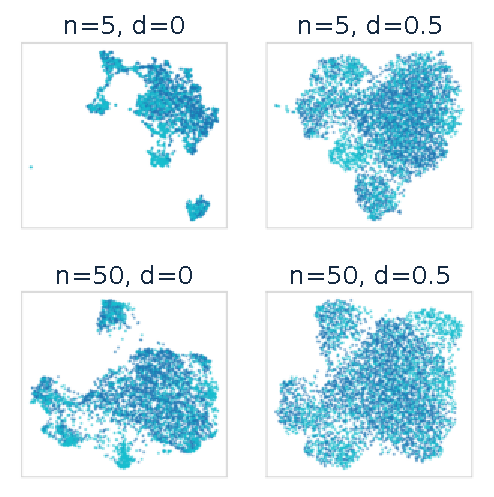
\includegraphics[width=.63\linewidth,height=62mm,keepaspectratio]{umap_selected.pdf}\end{center}
\figcaption{Figure 6. Four corners of the original sweep grid: small/large neighbourhood size and small/large min\_dist. Blue/cyan denote CMV-negative/positive donor labels. The full grid appears on two reserve slides.}

\topic{n\_neighbors: which scale of connectivity is modelled?}
A smaller neighbourhood emphasises very local relations and may separate groups connected only weakly at that scale. A larger neighbourhood brings more extended relations into the graph, often yielding a more connected or smoother arrangement. This is a scale choice, not a universal ordering from bad to good. It can also affect runtime because the graph contains more candidate edges.

\topic{min\_dist: how tightly can connected points pack?}
Smaller min\_dist allows tightly packed regions; larger values discourage this packing and tend to spread observations more evenly. This setting affects the low-dimensional shape of the attraction curve. A value of zero does not mean that every connected pair must collapse to the same coordinates. Larger min\_dist also does not automatically make between-island distances quantitatively faithful.\cite{umapparams}

\begin{center}\begin{tabular}{rrr}\toprule
$n_{\rm neighbors}$ & min\_dist & $T(15)$\\\midrule
5 & 0.0 & 0.890139\\
5 & 0.1 & 0.879145\\
30 & 0.0 & 0.877151\\
\bottomrule\end{tabular}
\end{center}
\figcaption{Table 3. Three highest saved Trustworthiness settings. The selected configuration is n\_neighbors=5, min\_dist=0.0. These are within-sweep scores, not a comparison against the final 40,000-cell metrics.}

The final parameter choice maximises the recorded Trustworthiness, not visual separation by CMV or a manually preferred number of islands. The fixed choice of 15 evaluation neighbours is independent of the UMAP graph size of 5 in the winning configuration. Holding the evaluation definition constant makes configurations comparable; it does not remove the need to explain what scale that evaluation probes.

The sweep does not investigate alternative distance metrics, output dimensions, graph-connectivity settings, initialisations or multiple seeds. These remain possible sensitivity analyses, not analyses that were performed. The slides therefore describe parameter effects illustrated by the recorded examples rather than a comprehensive optimisation of UMAP.

\clearpage
\section*{9. Local metrics: exact overlap versus rank-weighted errors}
Write $N_i^X(k)$ for the $k$ nearest neighbours of observation $i$ in a reference representation and $N_i^Y(k)$ for those in a map. Both exclude the observation itself. The notebook uses $k=15$.

\topic{kNN preservation (shared-neighbour fraction)}
\[
 R(k)=\frac1n\sum_i\frac{|N_i^X(k)\cap N_i^Y(k)|}{k}.
\]
This is symmetric when both neighbourhoods have the same size. It is bounded between zero and one, and identical representations must score one. Ten shared neighbours out of fifteen give a per-cell value of $10/15=0.667$. Jaccard similarity would instead divide by the union size, giving $10/(15+15-10)=0.5$. These names must not be used interchangeably.

The average gives equal weight to cells. In the 40,000-cell dataset, equal cell counts also give equal total weight to each donor. The 5,000-cell sweep is only approximately donor-balanced. Chance overlap for two independent random size-$k$ subsets of the other $n-1$ cells has expectation $k/(n-1)$, approximately 0.000375 here. This is a mathematical reference level, not a tested null distribution for these dependent biological data.

\topic{Trustworthiness}
Trustworthiness penalises neighbours that appear in the map but were not among the original $k$ neighbours. Let $r_X(i,j)$ be the rank of $j$ among the original neighbours of $i$:
\[
 T(k)=1-\frac{2}{nk(2n-3k-1)}
 \sum_i\sum_{j\in N_i^Y(k)\setminus N_i^X(k)}[r_X(i,j)-k].
\]
The normalisation gives a score in $[0,1]$ in its valid parameter range; scikit-learn requires $k<n/2$. A falsely introduced neighbour ranked 16th receives penalty 1 when $k=15$, whereas one ranked 1,000th receives penalty 985. Trustworthiness therefore distinguishes near misses from distant intrusions. It is directional because the reference supplies the ranks.\cite{trust}

High $T$ does not mean that the same proportion of neighbours was retained. For example, many replacements just beyond the original top-$k$ boundary can leave $T$ high while exact overlap is low. Thus the final t-SNE values $T\approx0.961$ and $R\approx0.223$ are not percentages of the same event and are not contradictory.

\topic{The implementation correction}
The original code requested 15 neighbours with \texttt{kneighbors()} and then removed the first column. Without explicit query data, scikit-learn already excludes each indexed cell itself, so this kept 14 real neighbours while still dividing by 15. A deterministic identical-input test returned $14/15$, exposing the error. The corrected helper retains all returned columns; tests also cover duplicates, one-neighbour queries, symmetry, a known overlap and invalid sizes.\cite{neighbors}

\clearpage
\section*{10. Global distances and separation by a clinical label}
\topic{Pearson correlation of pairwise distances}
For all unordered pairs within a fixed sample of 2,000 cells, let $a_{ij}=\lVert x_i-x_j\rVert$ in the 29-PC reference and $b_{ij}=\lVert y_i-y_j\rVert$ in a map. We compute
\[
 r_d=\frac{\sum_{i<j}(a_{ij}-\bar a)(b_{ij}-\bar b)}
 {\sqrt{\sum_{i<j}(a_{ij}-\bar a)^2}\sqrt{\sum_{i<j}(b_{ij}-\bar b)^2}}.
\]
There are $2{,}000\times1{,}999/2=1{,}999{,}000$ pair distances. Reusing the same sampled cells makes the three comparisons consistent. These pair distances are dependent, so their count should not be presented as the number of independent biological observations or used naively to justify a tiny significance level.

\begin{center}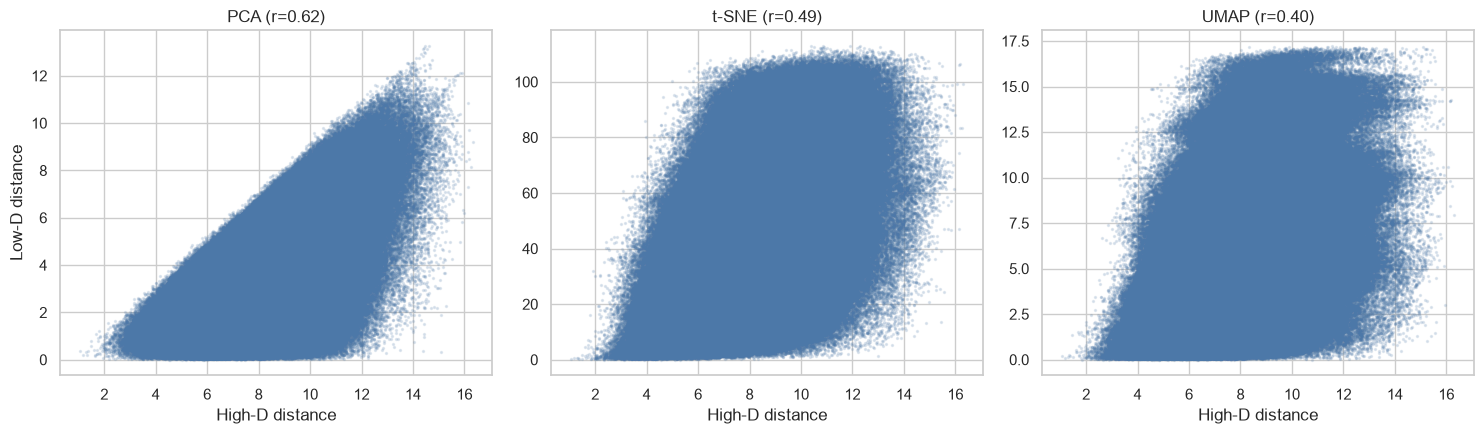
\includegraphics[width=\linewidth,height=46mm,keepaspectratio]{shepard.png}\end{center}
\figcaption{Figure 7. Saved Shepard diagrams: each point is a cell pair, not one cell. The x-axis is reference distance and the y-axis is distance in the respective map.}

An exact isometry gives the identity line; uniform rescaling gives another positive straight line with $r_d=1$. Correlation is insensitive to such rescaling, so a diagonal is not necessary for a perfect correlation. Nonlinear distortions and scatter reduce linear correspondence. The quantity here is Pearson correlation between distance vectors, not the separate statistical measure called distance correlation used to test dependence.

\topic{Silhouette by CMV status}
For cell $i$, $a(i)$ is its mean distance to other cells carrying the same donor CMV label; $b(i)$ is its mean distance to the other label group. The silhouette is
\[
 s(i)=\frac{b(i)-a(i)}{\max\{a(i),b(i)\}},\qquad
 S_{\rm CMV}=\frac1n\sum_i s(i).
\]
Values near one indicate well-separated labelled groups, near zero indicate little separation, and negative values indicate that cells are closer on average to the other group. The saved values here are only 0.0016--0.0178. UMAP has the largest numerical value, but all are small. This metric evaluates the geometry of these particular labels, not preservation of the original data structure.

\begin{center}\small\begin{tabular}{lrrrr}\toprule
Embedding & $T(15)\uparrow$ & $R(15)\uparrow$ & $r_d\uparrow$ & $S_{\rm CMV}\uparrow$\\\midrule
PCA & \worst{0.7258} & \worst{0.0072} & \best{0.6204} & \worst{0.0016}\\
t-SNE & \best{0.9612} & \best{0.2232} & 0.4868 & 0.0104\\
UMAP & 0.9009 & 0.1126 & \worst{0.3954} & \best{0.0178}\\
\bottomrule\end{tabular}
\end{center}
\figcaption{Table 4. Final 40,000-cell results. kNN values are corrected; Pearson correlations were verified against the committed 29-PC reference. Trustworthiness and silhouette remain saved notebook outputs, not fresh full-data computations. Green/red indicate numerical extrema within each column.}

\clearpage
\section*{11. Pairwise comparison: Procrustes as the task's chosen measure}
Comparing each embedding against a high-dimensional reference is different from comparing the embeddings to one another. The assignment explicitly asks for all pairs of visualizations. We choose Procrustes disparity as the primary pairwise measure and add corrected kNN overlap to show how the conclusion depends on the meaning of similarity.

Let $A,B\in\mathbb R^{n\times2}$ contain the same cells in the same order. Centre both maps and divide each by its Frobenius norm:
\[
 A_c=\frac{A-\bar A}{\lVert A-\bar A\rVert_F},\qquad
 B_c=\frac{B-\bar B}{\lVert B-\bar B\rVert_F}.
\]
SciPy's Procrustes disparity then measures
\[
 M^2=\min_{s,Q:\,Q^\top Q=I}\lVert A_c-sB_cQ\rVert_F^2.
\]
The orthogonal matrix $Q$ allows rotations and reflections; $s$ supplies a uniform scale adjustment. Translation was already removed by centring. These transformations are appropriate because map orientation, position and overall units are arbitrary. Different nonlinear layouts remain different even after this alignment. The scalar disparity is symmetric for this normalised problem, although the returned transformed coordinate matrices have different normalisation conventions.\cite{procrustes}

\begin{center}\begin{tabular}{lrr}\toprule
Pair & $R(15)\uparrow$ & $M^2\downarrow$\\\midrule
PCA vs t-SNE & 0.00585 & \best{0.45189}\\
PCA vs UMAP & \worst{0.00410} & \worst{0.73390}\\
t-SNE vs UMAP & \best{0.12532} & 0.72369\\
\bottomrule\end{tabular}
\end{center}
\figcaption{Table 5. All three pairs, using 40,000 corresponding cells. Larger $R(15)$ means more shared local neighbours; smaller $M^2$ means better globally aligned shape.}

\begin{center}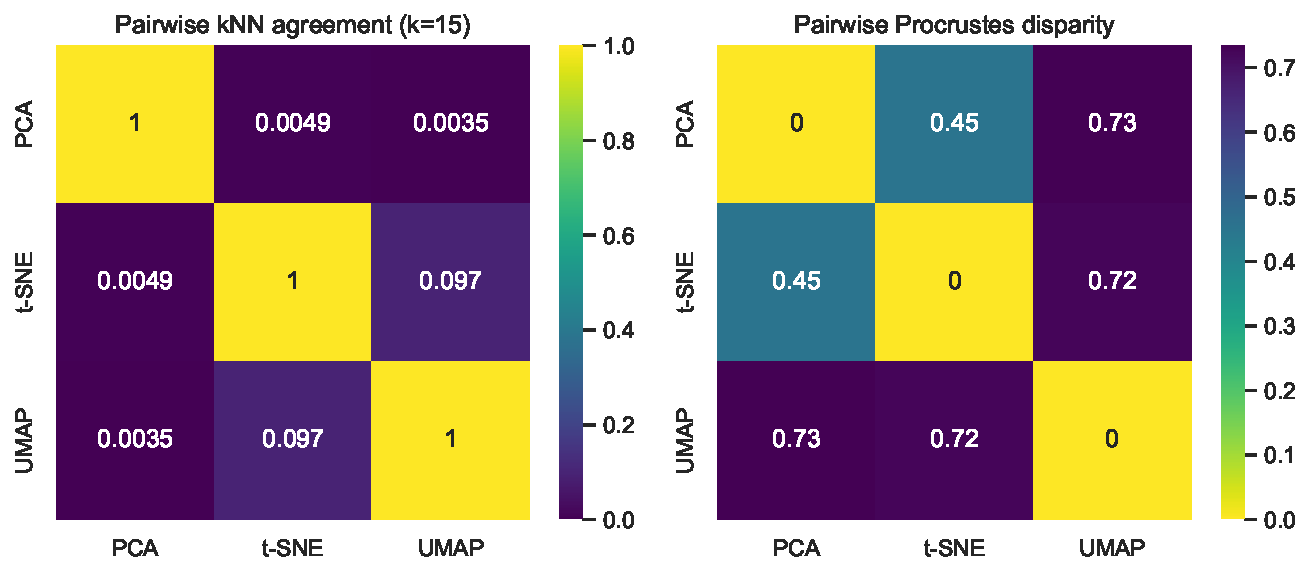
\includegraphics[width=.79\linewidth,height=55mm,keepaspectratio]{pairwise.pdf}\end{center}
\figcaption{Figure 8. The same corrected values as matrices. Diagonal entries are identity comparisons, not additional experiments.}

PCA--t-SNE has the lowest disparity (0.451891), while t-SNE--UMAP has the highest local overlap (0.125318). The latter is an average of approximately $15\times0.125318=1.88$ shared neighbours per cell, not 12.5\% agreement about clinical labels. PCA--UMAP has the lowest local overlap and the largest disparity among the tested pairs.

These conclusions are compatible: smooth distortions may preserve neighbourhoods while changing global shape; similar global outlines can still place individual cells next to different neighbours. Neither metric declares one embedding biologically correct. The same-row requirement is essential: permuting one matrix without matching the other would compare different cells and invalidate both calculations.

\clearpage
\section*{12. Marker overlays: biological hypotheses, not validated populations}
Colouring by CMV status asks whether the map separates cells according to a donor-level label. Colouring by individual marker expression asks a different question: where in a particular map a phenotype-related signal appears. The notebook displays NKG2C, CD57, CD56, CD16, CD19, TRAIL, CD25 and NKp44 on the saved UMAP and t-SNE maps.

\begin{center}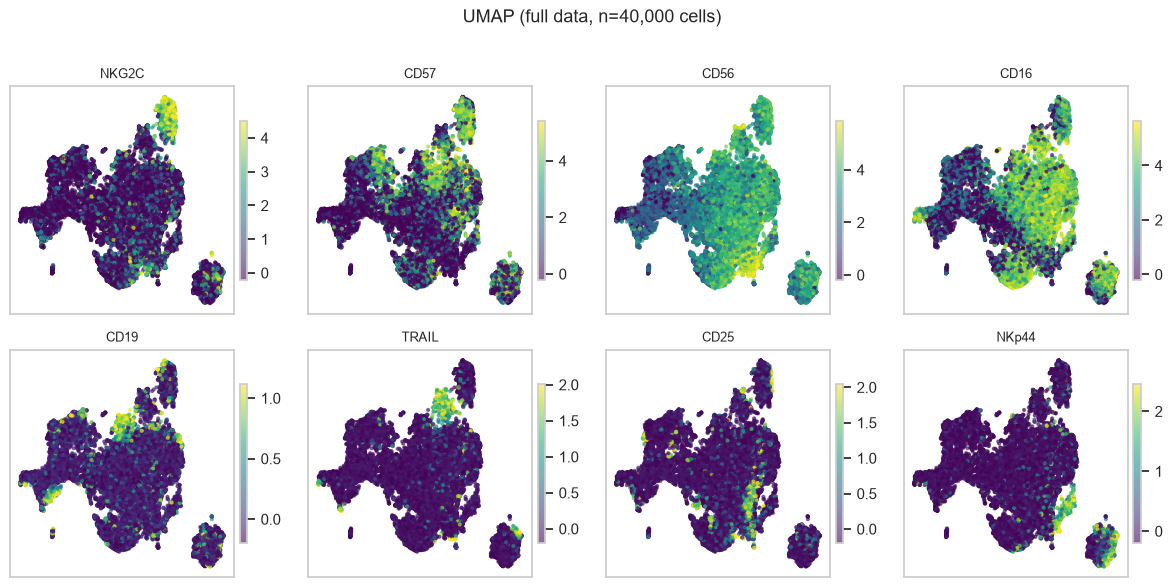
\includegraphics[width=\linewidth,height=76mm,keepaspectratio]{umap_markers.png}\end{center}
\figcaption{Figure 9. Original saved UMAP overlays (cell 41), based on all 40,000 cells in the balanced analysis sample. ``Full data'' in the original plot title refers to this analysis sample.}

NKG2C and CD57 are relevant to the memory-like NK phenotype discussed by Horowitz et al. CD56 and CD16 help place expression patterns in NK-cell context. Other markers provide additional checks on heterogeneity and interpretation. A region with high intensity for one marker does not establish that the same cells are high for another; co-expression requires comparing aligned cells or explicitly computing joint positivity.

The colour scale for each marker uses its own 1st and 99th percentiles of arcsinh-transformed values. This limits visual domination by extreme values but saturates the tails. Brightness therefore cannot be directly compared between different markers. The same marker's overlays are comparable across the two maps because they use the same underlying values and cells. Their locations can change because the embedding coordinates change.

\topic{How to phrase the observation}
An appropriate statement is that the maps provide candidate regions for examining marker combinations. An inappropriate conclusion would be that a visible island is a confirmed adaptive population, that those individual cells are infected, or that the map has established superior diagnostic performance. Confirmation would require a justified phenotype definition and additional biological or predictive validation.

The paired t-SNE panels are provided in the separate two-page appendix and on a reserve slide rather than repeating every large plot in the main text. No extra clustering was fitted to justify the visual interpretation, and no synthetic biological example was substituted for the saved marker outputs. The sampling check and overlays remain the notebook's exploratory evidence, with their thresholding and scaling limitations stated explicitly.

\clearpage
\section*{13. What was checked, what was retained, and how to reproduce it}
The source is \texttt{02\_dimensionality\_reduction\_clean.ipynb} from main commit \texttt{252415a}. A direct remote query confirmed that this was the latest pushed main when implementation began. Changes were made on the separate \texttt{slides-aufgabe-2} worktree branch; the other branch's running analysis was not used as an output location.

\begin{center}
\begin{tabular}{p{.38\linewidth}p{.54\linewidth}}\toprule
Item & Treatment for these documents\\\midrule
Raw input tables and stored coordinates & Read-only; metadata order, donor counts and PCA-coordinate alignment checked\\
PCA variance spectrum & Verified from covariance of the same transformed and standardised markers\\
Final kNN scores & Recalculated with exactly 15 neighbours excluding self\\
Procrustes and distance correlations & Checked from existing coordinates; fixed 2,000-cell sample for distances\\
t-SNE/UMAP models and sweep plots & Reused; no embedding training or sweep rerun\\
Trustworthiness and CMV silhouette & Retained saved outputs; no new full-data computation\\
GMM sampling-check plot & Retained original output; not a fresh gate validation\\\bottomrule
\end{tabular}
\end{center}

\topic{Why the reference is now explicit}
The notebook fitted 30 PCs and selected 29, but its quality-code reference still named the 30-PC variable. The currently saved Pearson correlations match the committed 29-PC array, not the 30-PC alternative. The reference now explicitly uses the selected 29 PCs. The kNN error was corrected independently: no first neighbour is discarded from the query with implicit training data. A full notebook rerun would recompute all sweep kNN values correctly; this delivery deliberately avoids those expensive training runs and removes the invalid saved columns instead.

\topic{Reproducing the small correction and the documents}
The reusable exporter reads the committed input tables and embeddings, verifies their alignment, requests neighbours with a 64 MiB working-memory setting, and exports document figures, tables and provenance. Its computations are constrained to one thread. The provenance file records input and notebook hashes, the seed, sample sizes, reference dimension and which quantities were recalculated. Running it does not call t-SNE or UMAP.

Compile the LaTeX documents with the included figures and tables; Python and the raw FCS files are not required for compilation. The slides load the existing parent presentation theme, with a local Task 2 footline override. A short README gives the exact commands and package requirements. The one-page report body is supplied without a document wrapper so it can be incorporated into the group report; the supplementary appendix remains a separate document.

\topic{Boundary with the later tasks}
This analysis gives candidate structure and quantifies projection differences. It does not replace donor-wise validation of CellCNN, Citrus and the linear single-cell SVM. In those comparisons, donors remain the independent observations, splits must be shared between methods, and fitted preprocessing must use training donors only. Clear separation of these claims allows the Task 2 section to fit coherently into the full project without overstating what its maps demonstrate.

\clearpage
\section*{14. References and source documentation}
\begingroup\small
\renewcommand{\refname}{}
\begin{thebibliography}{99}
\bibitem{horowitz} Horowitz, A. et al. (2013). Genetic and environmental determinants of human NK cell diversity revealed by mass cytometry. \emph{Science Translational Medicine}, 5, 208ra145. \href{https://pmc.ncbi.nlm.nih.gov/articles/PMC3918221/}{Full text and original study figures}.
\bibitem{cellcnn} Arvaniti, E. and Claassen, M. (2017). Sensitive detection of rare disease-associated cell subsets via representation learning. \emph{Nature Communications}, 8, 14825. \href{https://pmc.ncbi.nlm.nih.gov/articles/PMC5384229/}{Full text}.
\bibitem{tsne} van der Maaten, L. and Hinton, G. (2008). Visualizing data using t-SNE. \emph{Journal of Machine Learning Research}, 9, 2579--2605. \href{https://www.jmlr.org/papers/v9/vandermaaten08a.html}{Original paper}.
\bibitem{umap} McInnes, L., Healy, J. and Melville, J. (2018; revised 2020). UMAP: Uniform Manifold Approximation and Projection for Dimension Reduction. arXiv:1802.03426. \href{https://arxiv.org/abs/1802.03426}{Paper and versions}.
\bibitem{trust} Venna, J. and Kaski, S. (2001). Neighborhood preservation in nonlinear projection methods: an experimental study. \emph{ICANN 2001}, 485--491. Formula and implementation: \href{https://scikit-learn.org/stable/modules/generated/sklearn.manifold.trustworthiness.html}{scikit-learn Trustworthiness documentation}.
\bibitem{neighbors} scikit-learn. \href{https://scikit-learn.org/stable/modules/generated/sklearn.neighbors.NearestNeighbors.html}{NearestNeighbors documentation}, especially the \texttt{kneighbors(X=None)} self-exclusion convention.
\bibitem{tsneapi} scikit-learn. \href{https://scikit-learn.org/stable/modules/generated/sklearn.manifold.TSNE.html}{TSNE API documentation}: parameter meanings, learning-rate convention and implementation defaults.
\bibitem{pcaapi} scikit-learn. \href{https://scikit-learn.org/stable/modules/generated/sklearn.decomposition.PCA.html}{PCA API documentation}: component selection, solvers, whitening and explained variance.
\bibitem{umapparams} UMAP project. \href{https://umap-learn.readthedocs.io/en/latest/parameters.html}{Basic UMAP parameters}: neighbourhood size, minimum distance and distance metrics.
\bibitem{umapdocs} UMAP project. \href{https://umap-learn.readthedocs.io/en/latest/how_umap_works.html}{How UMAP works}: graph construction and mathematical background.
\bibitem{procrustes} SciPy. \href{https://docs.scipy.org/doc/scipy/reference/generated/scipy.spatial.procrustes.html}{scipy.spatial.procrustes}: normalisation, allowed transformations and returned disparity.
\end{thebibliography}
\endgroup
\topic{Primary computational source}
The cleaned notebook, exported arrays and labels committed in the repository are the source of the experimental settings and results. \texttt{data/provenance.json} identifies their exact hashes. The citations above explain methods and biological context; they do not independently verify the project's particular numerical outcomes.
\end{document}
